\documentclass[11pt]{article}

\usepackage[margin=1in]{geometry}
\usepackage{microtype}
\usepackage[T1]{fontenc}
\usepackage[utf8]{inputenc}
\usepackage{lmodern}

\usepackage{amsmath,amssymb}
\usepackage{booktabs}
\usepackage{enumitem}
\usepackage{xcolor}
\usepackage{hyperref}
\usepackage{graphicx}
\usepackage{tikz}
\usetikzlibrary{positioning,calc,arrows.meta}
\usepackage{listings}
\usepackage[numbers]{natbib}

% pandoc compatibility (used across projects)
\providecommand{\tightlist}{%
  \setlength{\itemsep}{0pt}\setlength{\parskip}{0pt}}

% Unicode support for common symbols
\DeclareUnicodeCharacter{2192}{\ensuremath{\rightarrow}} % →
\DeclareUnicodeCharacter{21D2}{\ensuremath{\Rightarrow}} % ⇒
\DeclareUnicodeCharacter{2264}{\ensuremath{\leq}} % ≤
\DeclareUnicodeCharacter{2265}{\ensuremath{\geq}} % ≥
\DeclareUnicodeCharacter{03C4}{\ensuremath{\tau}} % τ
\DeclareUnicodeCharacter{03F5}{\ensuremath{\epsilon}} % ϵ
\DeclareUnicodeCharacter{2208}{$\in$} % ∈

\hypersetup{
  colorlinks=true,
  linkcolor=blue,
  urlcolor=blue,
  citecolor=blue
}

\setlist[itemize]{leftmargin=*, itemsep=0.25em, topsep=0.25em}
\setlist[enumerate]{leftmargin=*, itemsep=0.25em, topsep=0.25em}

\lstset{
  basicstyle=\ttfamily\small,
  breaklines=true,
  frame=single,
  xleftmargin=1em,
  xrightmargin=1em
}

\begin{document}

\begin{titlepage}
\thispagestyle{empty}
\raggedright

\vspace*{0.62\textheight}

{\LARGE Phase Discipline for Regulated Agents\par}
\vspace{0.25em}
{\Large Transition Windows and State--Action Alignment\par}
\vspace{0.4em}
{\large\itshape Agent architectures / robotics / regulated discovery\par}

\vspace{1.6em}

Tyson Jeffreys\\
Independent Researcher\\
\href{mailto:tyson@staygolden.dev}{tyson@staygolden.dev}

\vspace{1.6em}

Version 0.1 --- February 12, 2026

\end{titlepage}

\noindent\textbf{Series note.} This paper extends the Baseline regulation series by naming a missing runtime layer: \emph{phase discipline}. Prior papers specify (i) a regulator layer with bands, budgets, rollback, and a telemetry-driven global restraint signal $g(t)$ for trustworthy discovery \citep{jeffreys2025baseline_constraint,jeffreys2026two_regime_control}; (ii) representation-level commits via concept containers \citep{jeffreys2026concept_containers}; (iii) a research-systems objective centered on reusable analysis artifacts and bursty synthesis \citep{jeffreys2026time_to_analysis}; and (iv) verifier-gap governance where learned critics are treated as sensors, with abstention as uncertainty telemetry and commits gated under non-verifiable selection \citep{provilkov2025escaping}. Here we add a second runtime control variable alongside posture: a phase state $p(t)$ that schedules work types and reserves transition windows for consolidation and commits.\par\medskip

\section*{Abstract}
Band-limited regulation constrains \emph{how risky} an agent may operate (budgets, allowed actions, rollback), but it does not specify \emph{when} different classes of cognitive work should occur. In practice, many failures are not outright constraint violations; they are \textbf{state--action mismatches}: deep planning during periods of high internal contention, commitment under unstable selection signals, or exploration when the system is already compensating.

We propose \textbf{phase discipline}: a runtime layer that tracks a small phase state $p(t)$ (restore, transition, act) and enforces \textbf{state--action alignment} by gating action classes, planning depth, and commit rights based on phase. The key primitive is the \textbf{transition window}: a stable interval reserved for consolidation (analysis artifacts), representation commits (concept containers), and policy updates, with \textbf{bounded override} as a priced, recoverable mechanism for deliberate phase-breaking.

We specify a minimal phase controller, relate it to Two-Regime Control (latent coordination vs. compensation), show how it composes with the global restraint signal $g(t)$ and verifier-gap selection telemetry, and propose measurable metrics and A/B experiments in tool-using and robotics settings.

\begin{center}\rule{0.5\linewidth}{0.5pt}\end{center}

\section{1. Motivation: beyond bands}
\subsection{1.1 The missing failure mode}
In \emph{Regulatory Ground}, trustworthy discovery is framed as a band-limited optimization problem: as capability and actuation increase, failures shift from isolated errors to cascades, and the agent requires an explicit regulator layer (bands, budgets, uncertainty gating, checkpoint/rollback, and safe mode) \citep{jeffreys2025baseline_constraint}. That layer controls \emph{risk posture} via a telemetry-driven global restraint signal $g(t)$.

However, many real failures arise even when $g(t)$ is conservative:
\begin{itemize}
\item \textbf{Thrash}: repeated recomputation and reversals (plan churn) without violating a hard constraint.
\item \textbf{Chronic compensation}: the system sustains a high-activation mode longer than necessary, accumulating error and fatigue-like artifacts \citep{jeffreys2026two_regime_control}.
\item \textbf{Premature commits}: durable writes (documents, policies, representations) made while selection is unstable or evidence is weak \citep{jeffreys2026concept_containers}.
\end{itemize}

These are not primarily ``unsafe actions''; they are \emph{operating discipline} failures. The system is doing the wrong kind of work at the wrong time.

\subsection{1.2 A second control variable}
We propose adding a second low-dimensional runtime controller:
\begin{itemize}
\item \textbf{Posture} $g(t)$: how tightly constrained the system should be (budgets, allowed actions, escalation).
\item \textbf{Phase} $p(t)$: what operating mode the system should be in (act, restore, transition), which determines what \emph{classes of work} are permitted now.
\end{itemize}

The core thesis:
\begin{quote}
\textbf{Trustworthy discovery requires not only band limits on risk but phase discipline that schedules work to minimize internal contention, bound compensation duty cycles, and reserve stable transition windows for commits.}
\end{quote}


\section{2. Definitions}
\subsection{2.1 Phase variable}
Let $p(t)$ be a discrete phase state. A minimal taxonomy:
\begin{itemize}
\item \textbf{Act}: high throughput execution (tool use, exploration, task completion).
\item \textbf{Restore}: quiescence/recovery (monitoring, low-cost maintenance, minimal tool actions).
\item \textbf{Transition}: a bounded window for consolidation and commits (analysis artifacts, representation updates, policy writes).
\end{itemize}

Optional extensions (implementation-dependent):
\begin{itemize}
\item \textbf{Override}: deliberate phase-breaking with tightened budgets and mandatory recovery.
\item \textbf{Safe mode}: regulator-enforced fallback (already present in Regulatory Ground).
\end{itemize}

\subsection{2.2 Action classes}
Phase discipline works by gating \emph{action classes}. Example classes:
\begin{itemize}
\item \textbf{Explore}: widen hypotheses, sample plans, gather evidence.
\item \textbf{Exploit/Execute}: commit to a plan, act on the environment/tools.
\item \textbf{Consolidate}: compress state into analysis artifacts (levers, predictions, falsifiers).
\item \textbf{Commit}: durable writes: external actions with side effects, policy updates, or representation commits (containers).
\end{itemize}

\subsection{2.3 State--action mismatch}
Define \textbf{state--action mismatch} as a situation where the agent executes an action class that is disallowed or high-cost for its current phase. Mismatch is distinct from constraint violation:
\begin{itemize}
\item constraints are about \emph{external safety / budgets};
\item mismatch is about \emph{internal stability / contention / thrash}.
\end{itemize}

Mismatch is the phase analog of Two-Regime Control's compensation regime: it is the condition under which the system tends to burn compute/energy and accumulate errors \citep{jeffreys2026waste_energy,jeffreys2026two_regime_control}.

\section{3. The transition window}
\subsection{3.1 Why transitions matter}
The transition window is the key new primitive. It is not merely ``rest'' and not merely ``execution.'' It is a bounded interval reserved for:
\begin{itemize}
\item \textbf{Consolidation}: producing analysis artifacts that expose causal structure and falsifiers (Time-to-Analysis) \citep{jeffreys2026time_to_analysis}.
\item \textbf{Commit gating}: permitting durable writes only when uncertainty telemetry is favorable.
\item \textbf{Representation commits}: creating/updating concept containers as stable compressed structure \citep{jeffreys2026concept_containers}.
\end{itemize}

Intuition: commits are cheapest and safest when internal contention is lowest. In the absence of verifiers, commits must be coupled to uncertainty telemetry (abstention/tie mass, disagreement, stability) rather than confidence narratives \citep{provilkov2025escaping}.

\subsection{3.2 Phase discipline as ``baseline operation'' for agents}
In the Baseline series, ``baseline'' means operating near a stable attractor with minimal chronic compensation. Phase discipline operationalizes this for agents by:
\begin{itemize}
\item bounding time spent in high-activation action phases,
\item enforcing recovery/quiescence,
\item and concentrating irreversible commitments into controlled windows.
\end{itemize}

\section{4. Composition with runtime regulation}
\subsection{4.1 Orthogonality: \texorpdfstring{$g(t)$}{g(t)} vs \texorpdfstring{$p(t)$}{p(t)}}
A simple way to compose them:
\begin{itemize}
\item $g(t)$ sets \emph{tightness}: budgets, allowed tools, maximum plan depth.
\item $p(t)$ sets \emph{work type}: what classes of work are allowed now (execute vs consolidate vs recover).
\end{itemize}

Example: the system can be in phase \textbf{Act} but with high restraint (tight posture)---allowing only short-horizon execution and forbidding irreversible writes. Conversely, the system can be in phase \textbf{Transition} with low restraint, enabling deeper consolidation and broader commit rights.

\subsection{4.2 Telemetry inputs}
Phase and posture should be driven by similar telemetry, but interpreted differently.

\textbf{Posture} $g(t)$ uses telemetry to answer: \emph{How risky is it to act?}

\textbf{Phase} $p(t)$ uses telemetry to answer: \emph{Is the system stable enough to consolidate/commit, or should it restore, or act?}

Candidate telemetry (existing and new):
\begin{itemize}
\item \textbf{Constraint proximity}: budget exhaustion, near-miss rates, safety-controller interventions (Regulatory Ground).
\item \textbf{Compensation index}: internal thrash proxies, reversal rate, tool-call churn (Two-Regime / Waste Energy).
\item \textbf{Selection uncertainty}: abstention/tie mass, disagreement entropy, judge stability (Verifier Gap / judge-as-sensor).
\item \textbf{Recovery markers}: whether the system returns to low-thrash operation after load.
\end{itemize}

\subsection{4.3 Hysteresis and dwell time}
Agents can change phase rapidly. That is a feature, but it introduces a known control hazard: \textbf{chattering}. Phase transitions should include:
\begin{itemize}
\item \textbf{hysteresis}: different thresholds for entering vs exiting phases,
\item \textbf{dwell-time constraints}: minimum time in a phase before switching again.
\end{itemize}
This mirrors Regulatory Ground’s emphasis on stability and avoiding oscillation in posture control.

\section{5. A minimal phase controller}
\subsection{5.1 Phase scheduler}
Define a phase scheduler:
\[
p(t) = \pi(\text{telemetry},\; g(t),\; \text{task context})
\]
where $\pi$ is a small state machine (or hybrid controller) with conservative transitions.

A minimal policy:
\begin{itemize}
\item Enter \textbf{Restore} when compensation markers rise (thrash, reversal rate) or when budgets approach limits.
\item Enter \textbf{Transition} after restore when stability markers return (low thrash, stable selection telemetry).
\item Enter \textbf{Act} after transition when the next action is defensible (adequate evidence, low uncertainty).
\end{itemize}

\subsection{5.2 State machine sketch}
\begin{center}
\begingroup\catcode`\#=12\relax
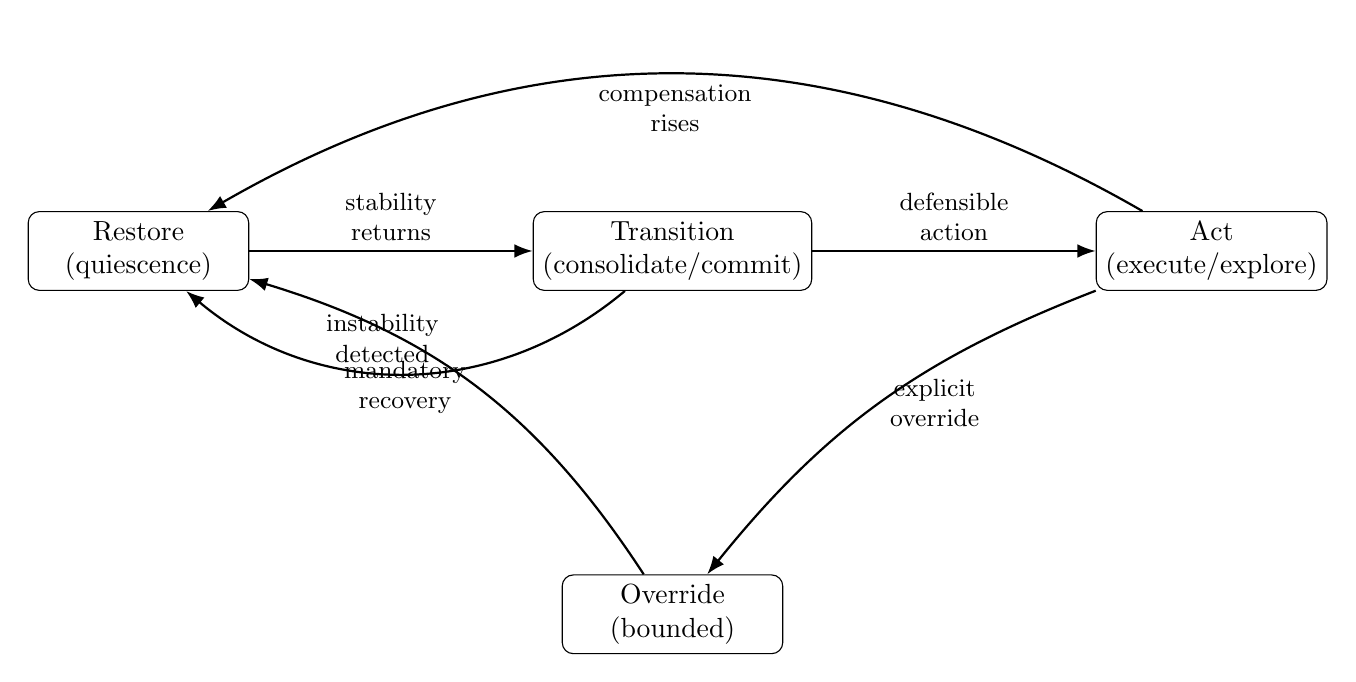
\begin{tikzpicture}[
  node distance=36mm,
  box/.style={draw, rounded corners, align=center, minimum width=28mm, minimum height=10mm},
  arrow/.style={-Latex, thick}
]
\node[box] (restore) {Restore\\(quiescence)};
\node[box, right=of restore] (transition) {Transition\\(consolidate/commit)};
\node[box, right=of transition] (act) {Act\\(execute/explore)};
\node[box, below=of transition] (override) {Override\\(bounded)};

% Forward progression
\draw[arrow] (restore) -- node[above,align=center,font=\small]{stability\\returns} (transition);
\draw[arrow] (transition) -- node[above,align=center,font=\small]{defensible\\action} (act);

% Return paths are curved to avoid label/box overlap.
\draw[arrow] (act) to[bend right=30] node[below,align=center,font=\small]{compensation\\rises} (restore);
\draw[arrow] (transition) to[bend left=40] node[above,align=center,font=\small,pos=0.55]{instability\\detected} (restore);

% Override branch
\draw[arrow] (act) to[bend right=15] node[right,align=center,font=\small]{explicit\\override} (override);
\draw[arrow] (override) to[bend right=20] node[left,align=center,font=\small]{mandatory\\recovery} (restore);
\end{tikzpicture}
\endgroup
\endgroup

\end{center}

\subsection{5.3 Action gating table}
\sloppy
A simple action-permission matrix:
\fussy

\begin{center}
\begin{tabular}{lccc}
\toprule
Action class & Restore & Transition & Act \\
\midrule
Monitor / low-cost checks & \checkmark & \checkmark & \checkmark \\
Evidence gathering (bounded) & \(\sim\) & \checkmark & \checkmark \\
Deep planning / broad search & \(\times\) & \(\sim\) & \checkmark \\
Consolidation (analysis artifacts) & \(\sim\) & \checkmark & \(\sim\) \\
Durable commits (writes/containers/policy) & \(\times\) & \checkmark\(^\dagger\) & \(\times\) \\
\bottomrule
\end{tabular}

\vspace{0.4em}
{\small \(^\dagger\)Commit is gated by uncertainty telemetry and posture: if abstention/tie mass is high, commits are blocked and evidence is required.}
\end{center}

\section{6. Bounded override}
\subsection{6.1 Why override exists}
Discovery often requires short deviations from phase alignment: pushing a difficult plan through, taking an expensive measurement, or exploring a risky branch. Phase discipline should not prohibit this; it should \emph{price and bound} it.

\subsection{6.2 Override policy}
Override is an explicit mode with:
\begin{itemize}
\item a declared objective and time budget,
\item tightened posture $g(t)$ (reduced tool rights, capped depth),
\item and a mandatory recovery path (return to Restore, then Transition).
\end{itemize}

Override is the macro analog of Two-Regime Control’s compensation regime: it is sometimes useful, but it must be duty-cycle bounded and recoverable \citep{jeffreys2026two_regime_control}.

\subsection{6.3 Required disclosure}
In verifier-free settings, override should emit a standardized disclosure block before non-trivial actions:
\begin{itemize}
\item what is being overridden (phase alignment),
\item what uncertainty is present,
\item what the bounded budget is,
\item and what recovery/rollback is available.
\end{itemize}
This mirrors the operating disclosure invariant introduced in Regulatory Ground and strengthened by judge-as-sensor telemetry.

\section{7. Commits as regulated events}
\subsection{7.1 Commit types}
A \textbf{commit} is any irreversible or persistent change:
\begin{itemize}
\item external writes with side effects,
\item policy/config updates that alter future behavior,
\item representation writes (concept container create/update),
\item long-lived analysis artifacts used as downstream inputs.
\end{itemize}

\subsection{7.2 Commit gating in the transition window}
Phase discipline proposes a simple rule:
\begin{quote}
\textbf{Commits are only permitted in Transition, and only when uncertainty telemetry is favorable.}
\end{quote}

This ties together:
\begin{itemize}
\item \textbf{Concept Containers}: container writes are commits \citep{jeffreys2026concept_containers}.
\item \textbf{Time-to-Analysis}: analysis artifacts are reusable structure; they should be produced when stable \citep{jeffreys2026time_to_analysis}.
\item \textbf{Verifier Gap}: if tie/abstain mass is high, do not commit---seek discriminating evidence \citep{provilkov2025escaping}.
\end{itemize}

\section{8. Implementation sketches}
\subsection{8.1 Tool-using research agent}
A regulated research agent can be structured as:
\begin{itemize}
\item Act: bounded evidence gathering and tool calls (search, fetch, parse).
\item Restore: low-cost monitoring and inventory of uncertainty.
\item Transition: produce analysis artifacts, run bounded selection (tournament), and commit a container or recommendation if permitted.
\end{itemize}

\subsection{8.2 Robotics: action vs consolidation}
In robotics, phase discipline maps naturally onto multi-rate stacks:
\begin{itemize}
\item high-rate control continues continuously,
\item low-rate planners and policy updates are phase gated,
\item commits (map updates, policy changes) are reserved for stable windows.
\end{itemize}

The transition window is where to perform:
\begin{itemize}
\item map/scene consolidation,
\item belief revision after contradictions,
\item safe policy updates,
\item and checkpointing.
\end{itemize}

\section{8. Implementation sketches}
\subsection{8.1 Tool-using research agent}
A regulated research agent can be structured as:
\begin{itemize}
\item Act: bounded evidence gathering and tool calls (search, fetch, parse).
\item Restore: low-cost monitoring and inventory of uncertainty.
\item Transition: produce analysis artifacts, run bounded selection (tournament), and commit a container or recommendation if permitted.
\end{itemize}

\subsection{8.2 Robotics: action vs consolidation}
In robotics, phase discipline maps naturally onto multi-rate stacks:
\begin{itemize}
\item high-rate control continues continuously,
\item low-rate planners and policy updates are phase gated,
\item commits (map updates, policy changes) are reserved for stable windows.
\end{itemize}

The transition window is where to perform:
\begin{itemize}
\item map/scene consolidation,
\item belief revision after contradictions,
\item safe policy updates,
\item and checkpointing.
\end{itemize}

\section{9. Metrics and experiments}
\subsection{9.1 Metrics}
Phase discipline enables new measurable quantities:
\begin{itemize}
\item \textbf{Phase mismatch rate}: fraction of actions executed in disallowed/high-cost phases.
\item \textbf{Override duty cycle}: time in override divided by wall time.
\item \textbf{Recovery half-life}: time to return to low-thrash operation after override.
\item \textbf{Commit timing quality}: commits per stable-transition window vs commits in act/restore.
\item \textbf{Thrash reduction}: reversal count, tool-call churn, plan variance (Waste Energy / Two-Regime proxies).
\item \textbf{Novelty yield under regulation}: durable novelty per unit of override budget (Regulatory Ground evaluation style).
\end{itemize}

\subsection{9.2 A/B tests}
Two simple experiments:
\begin{enumerate}
\item \textbf{Phase discipline on/off}: same agent, same tools, same tasks; only phase gating differs. Measure thrash, commit error rate, and recovery.
\item \textbf{Commit-in-transition vs commit-anytime}: allow container writes and policy updates only in Transition vs anywhere. Measure contamination (revision half-life, reversal count) and downstream performance.
\end{enumerate}

\section{10. Discussion: ``harmonic'' operation is not benevolence}
Phase discipline pushes systems toward lower oscillation, lower thrash, and bounded compensation duty cycles. This can look like ``harmonic'' behavior: stable trajectories with rapid recovery after perturbation.

But \textbf{harmonic operation is not a moral guarantee}. Benevolence still depends on:
\begin{itemize}
\item the invariants and objectives the regulator enforces,
\item commit governance (what the system is allowed to change),
\item and traceability/auditability.
\end{itemize}

The correct claim is narrower and testable: \emph{phase discipline reduces internal contention and makes discovery more sustainable and recoverable.}

\section{11. Conclusion and next steps}
We introduced phase discipline as a missing runtime layer in regulated agents: a discrete phase variable $p(t)$ that schedules work types and reserves transition windows for consolidation and commits. It composes naturally with the global restraint signal $g(t)$ (risk posture) and with verifier-gap governance (judge-as-sensor uncertainty telemetry).

Immediate next steps:
\begin{enumerate}
\item Add a phase mismatch failure mode and phase metrics to the Regulatory Ground benchmark harness.
\item Patch Concept Containers to make abstention-gated container writes explicit (commit as regulated event).
\item Implement a minimal phase scheduler in a tool-using agent and measure thrash reduction and commit quality.
\item Extend to robotics stacks by phase-gating low-rate planning and durable updates.
\end{enumerate}

\bibliographystyle{unsrtnat}
\bibliography{refs}

\section*{Note on authorship and tools}
This work was developed through iterative reasoning, modeling, and synthesis. Large language models were used as a
collaborative tool to assist with drafting, clarification, and cross-domain translation. All conceptual framing,
structure, and final judgments remain the responsibility of the author.

\end{document}
